\documentclass[A4paper, 11pt]{article}
\usepackage[slovene]{babel}
\usepackage[utf8]{inputenc}
\usepackage{array}
\usepackage{amsfonts}
\usepackage{amsmath}
\usepackage{pifont}
\usepackage{theorem}
\usepackage{authblk}
\usepackage{url}
\usepackage[normalem]{ulem}

\usepackage{graphicx}
\usepackage{subcaption}
\graphicspath{ {slike/} }

\title{Seminarska naloga iz statistike}
\author{Klementina Pirc}
\affil{Fakulteta za matematiko in fiziko \\ Oddelek za matematiko}
\date{julij 2020}

\newtheorem{definicija}{Definicija}
\theorembodyfont{\mdseries}
\newtheorem{zgled}{Zgled}

\newcommand{\cmark}{\ding{51}}
\newcommand{\xmark}{\ding{55}}

\begin{document}

\begin{titlepage} 

\maketitle
\thispagestyle{empty}
	
\end{titlepage}

Podrobnejša navodila nalog se nahajajo v datoteki \textit{27\_sem\_nal\_Klementina\_Pirc.pdf}

% 1. NALOGA

\section*{1. naloga}

V datoteki \textit{Kibergrad.csv} so podane informacije o 43 886 družinah. Spodnje naloge se navezujejo na stopnjo izobrazbe, ki jo imajo vodje gospodinjstev. Stopnje so označene s števili od 31 do 46. Naloge sem rešila s pomočjo programa Python in ustreznih knjižnic, postopek pa se nahaja v datoteki \textit{Kibergrad.py}

\subsection*{a)}
Na podlagi enostavnega slučajnega vzorca 200 družin poiščemo oceno za delež družin v celotni populaciji, katerih vodja gospodinjstva nima srednješolske izobrazbe. S pomočjo opisov stopenj izobrazbe ugotovimo, da moramo prešteti družine iz vzorca s stopnjo $<= 38$. Naj bo $d_i$ stopnja izobrazbe za i-to družino, definiramo 
\[x_i = \left \{
	\begin{array}{ll}
		1  & \mbox{če } d_i \leq 38 \\
		0 & \mbox{sicer}
	\end{array}
	\right.
\]
Sedaj lahko vzorčni delež $s$ izračunamo s formulo
\[ s = \frac{1}{n} \sum_{i=1}^{n} x_i \]
kjer je $n$ velikost vzorca, torej 200. Dobimo rezultat $s = 0.23$.  

\subsection*{b)}
Ocenimo standardno napako $se(s)$ in določimo 95\% interval zaupanja. Za izračun standardne napake moramo izračunati varianco $s$. Ker smo vzeli enostavni slučajno vzorec velja
\[ var(s) = \frac{1}{n} \frac{N - n}{N - 1} \tilde{\sigma}^2 \]
kjer je $N=43886$ velikost populacije in $\tilde{\sigma}^2$ nepristranska cenilka za populacijsko varianco. Torej
\[ 
\begin{split}
\tilde{\sigma}^2 = \frac{N - 1}{N (n - 1)} \sum_{i=1}^{n} (x_i - s)^2 \\
\Rightarrow var(s) & = \frac{N - n}{n N (n - 1)} \sum_{i=1}^{n} (x_i - s)^2 \\
		         & = \frac{N - n}{n N (n - 1)} \sum_{i=1}^{n} (x_i^2 - 2x_i s + s^2) \\
		         & = \frac{N - n}{n N (n - 1)} \sum_{i=1}^{n} (x_i - 2x_i s + s^2) \\
		         & = \frac{N - n}{N (n - 1)} (s - s^2)
\end{split}
\]
in zato
\[ se(s) = \sqrt{ \frac{N - n}{N (n - 1)} s (1 - s)} \]
Upoštevali smo $x_i ^2 = x_i$, kar velja, ker $x_i \in \{0,1\}$. Standardna napaka za izbrani vzorec je $0.029763$. \\
\\ % naved knjigo kot vir
Interval zaupanja dobimo po formuli $s \mp z_\alpha se(s)$. Ker želimo 95\% natančnost, je $z_\alpha = 1.96$ in tako dobimo interval $[0.171662, 0.288337]$.

\subsection*{c)}
Izračunamo populacijski delež $S$ in standardno napako $se(S)$ s formulama
\[ S = \frac{1}{N} \sum_{i=1}^{N} x_i  \qquad se(S) = \sqrt{\frac{\sigma ^2}{N}} = \sqrt{\frac{1}{N^2} \sum_{i=1}^{N} (x_i - S)^2} \]
ter dobimo $S=0.211502$ in $se(S)=0.001949$. Interval zaupanja torej pokrije populacijski delež, saj $S \in [0.171662, 0.288337]$. \\
\\
Razlika med vzorčnim in populacijskim deležem znaša $0.018497$, razlika med vzorčno in populacijsko standardno napako pa $0.027814$.

\subsection*{d)}
Izberemo še 99 vzorcev, določimo 95\% intervale zaupanja, ter jih narišemo skupaj z intervalom za prvi vzorec. S horizontalno črto označimo vrednost S. Vidimo, da populacijski delež pokrije 96 intervalov.

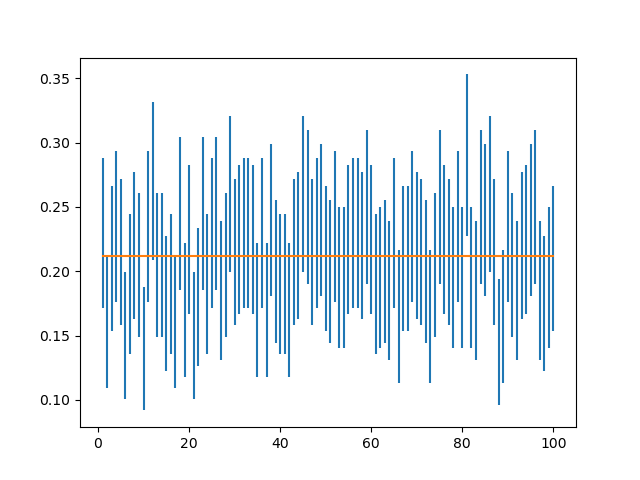
\includegraphics[scale=0.8]{Kibergrad_1}

\subsection*{e)}
Izračunamo standardni odklon vzorčnih deležev  iz 100 prej izbranih vzorcev. Uporabimo formulo
\[ \sigma_s = \sqrt{\frac{1}{m} \sum_{i=1}^{m} (s_i - \bar{s})^2} \] 
kjer je $m=100$ število vzorcev, $s_i$ vzorčni delež i-tega vzorca in $\bar{s}$ povprečje vzorčnih deležev. 
$\sigma_s = 0.028618$, razlika med populacijsko standardno napako $se(S)$ in $\sigma_s$ pa je 0.026668. 
% za vzorec velikosti 200?

\newpage

\subsection*{f)}
Sedaj izberemo 100 vzorcev velikosti 800 in ponovimo postopke iz točk d) in e).
\begin{itemize}
\item $\sigma_s = 0.013002$
\item $| \sigma_s - se(S) | = 0.011053$
\item populacijski delež S pokrije 95 intervalov zaupanja
\end{itemize}
% teli intervali so mal shady
% obrazlozitev in primerjava

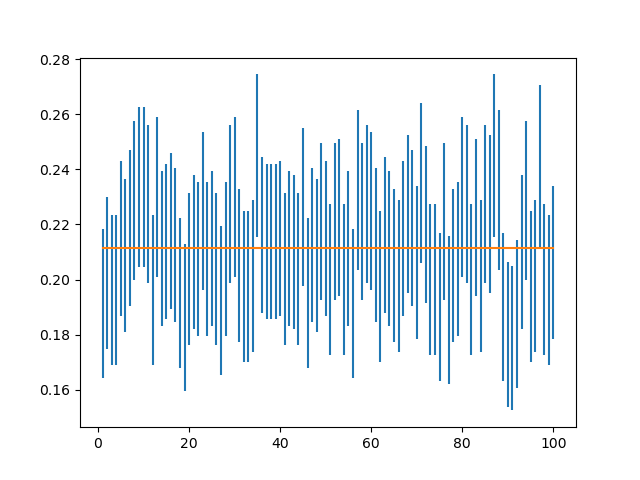
\includegraphics[scale=0.8]{Kibergrad_2}


% 2. NALOGA

\section*{2. naloga}

Želimo oceniti skupno vrednost inventarja z N enotami, kjer ima vsaka knjigovodsko vrednost $X$ in dejansko vrednost $Y$. Poznamo $X$ za vse enote in želimo oceniti vsoto dejanskih vrednosti vseh enot $\tau_Y$.
\[ \tau_Y = \sum_{i=1}^{N} Y_i \]
Vzamemo enostavni slučajni vzorec z $n$ enotami in predlagamo 3 možne cenilke

\[ \hat{\tau}_Y ^ {(0)} := N  \bar{Y} \qquad \hat{\tau}_Y ^ {(1)} := \tau_X + N ( \bar{Y} - \bar{X}) \qquad \hat{\tau}_Y ^ {(2)} := \frac{\bar{Y}}{\bar{X}} \tau_X \]

\subsection*{a)}
Dokažimo, da je $\hat{\tau_Y} ^ {(1)}$ nepristranska: $\dashuline{ E(\hat{\tau}_Y ^ {(1)}) = \tau_Y}$ in izračunajmo njeno varianco. Uporabili bomo naslednje oznake. \\
\\
$\tau_X$, $\tau_Y$ \ldots vsota vrednosti spremenljivke $X$ oz. $Y$ na celotnem inventarju, \\
$\mu_X$, $\mu_Y$ \ldots povprečna vrednost $X$ oz. $Y$ na celotnem inventarju, \\
$\sigma_X$, $\sigma_Y$ \ldots standardni odklon $X$ oz. $Y$ na vseh enotah inventarja, \\
$\rho_{XY}$ \ldots korelacijski koeficient med $X$ in $Y$ na celotnem inventarju, \\
$\bar{X}$, $\bar{Y}$ \ldots vzorčno povprečje $X$ oz. $Y$.


\[ 
\begin{split}
E(\hat{\tau}_Y ^ {(1)}) & = E(\tau_X + N (\bar{Y} - \bar{X})) \\
			       & = \tau_X  + N (E(\bar{Y}) - E(\bar{X})) \\
			       %& = \tau_X + N  \left ( \frac{1}{n} \sum_{i=1}^{n} ( E(Y_i) - E(X_i) ) \right ) \\ 
			       %& = \tau_X + N \left ( \frac{1}{n} \sum_{i=1}^{n} (\mu_Y - \mu_X) \right ) \\
			       & = \tau_X + N \mu_Y - N \mu_X \\
			       & = \tau_X + \tau_Y - \tau_X \\
			       & = \tau_Y
\end{split}
\]

\[
\begin{split}
var(\hat{\tau}_Y ^ {(1)})  & = var(\tau_X + N (\bar{Y} - \bar{X})) \\
				& = N^2 var( \bar{Y} - \bar{X} ) \\
				& = N^2 var( \bar{Y} + \bar{X} - 2 cov(\bar{Y},\bar{X}) ) \\
				& = N^2 ( \frac{\sigma_Y^2}{n} \frac{N - n}{N - 1} + \frac{\sigma_X^2}{n} \frac{N - n}{N - 1} - 2\rho_{XY} ) \\
				&= \frac{N^2}{n} \frac{N - n}{N - 1} (\sigma_Y^2 + \sigma_X^2) - 2 N^2 \rho_{XY}
\end{split}
\]

\subsection*{b)}
Privzamemo, da sta $X$ in $Y - X$ na populacijii neodvisni. Zanima nas, kdaj ima cenilka $\hat{\tau}_Y ^ {(1)}$ nižjo varianco kot cenilka $\hat{\tau}_Y ^ {(0)}$.

\[
\begin{split}
var(\hat{\tau}_Y ^ {(0)}) & = var(N \bar{Y}) \\
                                          & = \frac{N^2}{n} \frac{N - n}{N - 1} \sigma_Y^2
\end{split}
\]
\\
\[
\begin{split}
var(\hat{\tau}_Y ^ {(1)}) & < var(\hat{\tau}_Y ^ {(0)}) \\
 \frac{N^2}{n} \frac{N - n}{N - 1} (\sigma_Y^2 + \sigma_X^2) - 2 N^2 \rho_{XY} & < \frac{N^2}{n} \frac{N - n}{N - 1} \sigma_Y^2 \\
 \frac{N^2}{n} \frac{N - n}{N - 1} \sigma_X^2 - 2 N^2 \rho_{XY} & < 0 \\
 \frac{N^2}{n} \frac{N - n}{N - 1} \sigma_X^2 - 2 \frac{N^2}{n} \frac{N - n}{N - 1} \sigma_X^2 & < 0 \\
 - \frac{N^2}{n} \frac{N - n}{N - 1} \sigma_X^2  & < 0 \\
\end{split}
\]

To je očitno res, saj je $\sigma_X^2 > 0$ in zato $var(\hat{\tau}_Y ^ {(1)}) < var(\hat{\tau}_Y ^ {(0)}) $ velja vedno.
Zgoraj smo upoštevali še
\[
\begin{split}
cov(\bar{X}, \bar{Y}) & = cov(\bar{X}, \bar{Y} - \bar{X} + \bar{X}) \\
                                   & = cov(\bar{X}, \bar{Y} - \bar{X}) + cov(\bar{X}, \bar{X}) \\
                                   & = 0 + var(\bar{X}) \\
                                   & = \frac{\sigma_X^2}{n} \frac{N - n}{N - 1}
\end{split}
\]


% 3. NALOGA

\section*{3. naloga}

V datoteki \textit{Kiti.csv} so podani časi $t_1, \ldots, t_{210}$ za 210 kitov. i-ti kit v času $t_i$ preplava 1 km. Nalogo sem reševala s pomočjo programa Matlab, postopek pa se nahaja v datoteki \textit{Kiti.m}.

\subsection*{a)}
Narišemo histogram za dane podatke s pomočjo vgrajene funkcije \textit{histogram}. Širino razredov določimo glede na navodila in dobimo 
\[ l = \frac{2(q_{3/4} - q_{1/4})}{\sqrt[3]{n}} = 0.1141 \doteq 0.1 \]
kjer sta $q_{1/4}$, $q_{3/4}$ prvi in tretji kvartil, $n$ pa število podatkov.

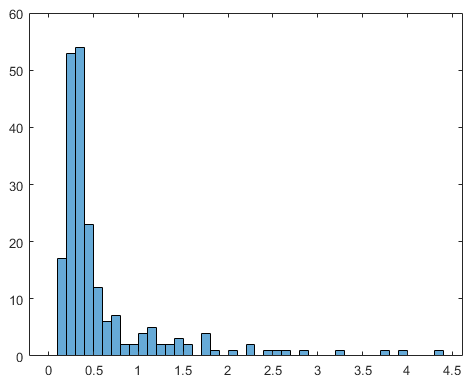
\includegraphics[scale=0.8]{Kiti_1}
\\
Glede na dobljeni histogram, se porazdelitev gama zdi ustrezna izbira za statistični model.

\subsection*{b)}
Radi bi ocenili parametra $\lambda$ in $\alpha$  porazdelitve $\gamma$ po metodi momentov. Pomagamo si s poglavjem 8.4 v knjigi. Na strani 260 izvemo, da je k-ti moment enak
\[ \mu_k = E(t^k) \quad k \in \mathbb{N} \]
kjer je $t$ slučajna spremenljivka. Oceno za $\mu_k$ pa lahko dobimo s pomočjo podanih podatkov kot
\[ \hat{\mu}_k = \frac{1}{n} \sum_{i=1}^{n} t_i^k \]
Ker imamo dva neznana parametra bomo potrebovali $\mu_1$ in $\mu_2$ za $\gamma$ porazdelitev. Najdemo ju na strani 263.
\[ \mu_1 = E(t) = \frac{\alpha}{\lambda} \qquad \mu_2 = E(t^2) = \frac{\alpha (\alpha + 1)}{\lambda^2} \]
Enačbi preoblikujemo in dobimo predpisa za $\lambda$ in $\alpha$
\[ \lambda = \frac{\mu_1}{\mu_2 - \mu_1^2} \qquad \alpha = \frac{\mu_1^2}{\mu_2 - \mu_1^2} \]
Z ocenami za $\mu_1$ in $\mu_2$ dobimo oceni $\hat{\lambda} = 1.3188$ in $\hat{\alpha} = 0.7992$. 

\subsection*{c)}
Ocenimo sedaj  $\lambda$ in $\alpha$ še po metodi največjega verjetja. Logaritemska funkcija verjetja je 
\[
\begin{split}
\ell (\lambda, \alpha | t_1, \ldots, t_n) & = \sum_{i=1}^{n} \log{\gamma(t_i)} \\
                                                              & = \sum_{i=1}^{n} (\alpha \log{\lambda} + (\alpha - 1) \log{t_i} - \lambda t_i - \log{\Gamma (\alpha)})
\end{split}
\]
Odvajamo $\ell$ in enačimo z 0, da dobimo cenilki za $\lambda$ in $\alpha$
\[
\begin{split}
\frac{\partial \ell}{\partial \lambda} & = \frac{n \alpha}{\lambda} + 0 - \sum_{i=1}^{n} t_i - 0 = 0 \\
\Rightarrow \qquad \hat{\lambda} & = \frac{n \alpha}{\sum_{i=1}^{n} t_i} \\
\\
\frac{\partial \ell}{\partial \alpha} & = n \log{\lambda} + \sum_{i=1}^{n} \log{t_i} - 0 - n \frac{\partial \log{\Gamma (\alpha)}}{\partial \alpha} = 0 \\
\Rightarrow \qquad 0 & =  n \log{\frac{n \alpha}{\sum_{i=1}^{n} t_i}} + \sum_{i=1}^{n} \log{t_i} - n \psi(\alpha) \\
\end{split}
\]
kjer je $\psi$ funkcija digama, ki je logaritemski odvod funkcije gama. Enačbo za cenilko $\alpha$ rešimo z vgrajeno funkcijo \textit{fzero}, ki sprejme funkcijo, začetni približek in vrne približek za ničlo funkcije, ki je v našem primeru ravno cenilka za $\alpha$. $\hat{\alpha}$ nato vstavimo v enačbo za $\hat{\lambda}$. Dobimo $\hat{\lambda} = 2.6327$ in $\hat{\alpha} = 1.5954$. \\
\\
Oceni parametrov se glede na metodo ocenjevanja precej razlikujeta. Navadno je metoda največjega verjetja bolj točna.

\subsection*{d)}
Na histogram dorišemo porazdelitvi $\gamma$ z dobljenimi ocenami za $\lambda$ in $\alpha$. Rdeč graf nam da metoda momentov, rumenega pa metoda največjega verjetja. Porazdelitvi se podatkom ne prilegata najbolje.

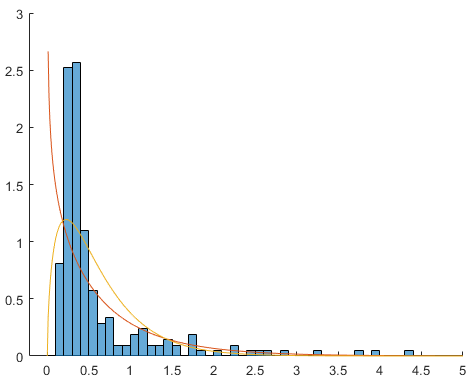
\includegraphics[scale=0.8]{Kiti_2}


\subsection*{e)}
Histogram in porazdelitvi narišemo še na logaritemski lestvici. Prileganje porazdelitev podatkom ni bistveno boljše kot prej.

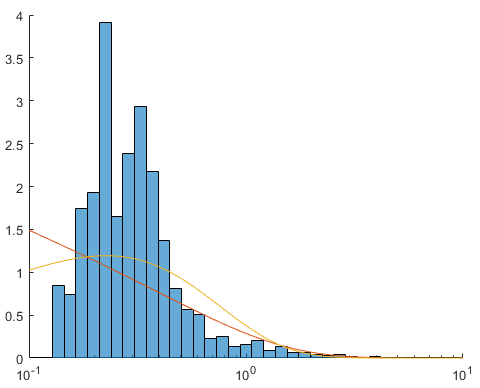
\includegraphics[scale=0.8]{Kiti_3}


% 4. NALOGA

\section*{4. naloga}

V datoteki \textit{TempPulz.csv} so podatki o telesni temperaturi in številu srčnih utripov na minuto za 65 moških in 65 žensk. Temperatura in utripi so porazdeljeni normalno. Nalogo sem reševala s pomočjo programa Matlab, postopek pa se nahaja v datoteki \textit{TempPulz.m}.

\subsection*{a)}
Oceniti želimo povprečja in standardne odklone za oba telesna parametra moških in žensk. Ocene bomo konstruirali na podlagi danih podatkov. Ločimo jih glede na spol, ter za obe skupini izračunamo povprečje in standardni odklon temperature in števila utripov.
Dobimo naslednje rezultate:
\begin{itemize}
\item povprečna temperatura moških je 98.1046$^{\circ}F$, žensk pa 98.3938$^{\circ}F$,
\item povprečni pulz moških je 73.3692, žensk pa 74.1538 utripov na minuto,
\item standardni odklon temperature pri moških je 0.6934$^{\circ}F$ in pri ženskah 0.7377$^{\circ}F$,
\item standardni odklon srčnega utripa pri moških je 5.8298 in pri ženskah 8.0426 udarcev na minuto. 
\end{itemize}

\subsection*{b)}
Za prej dobljena povprečja določimo 95\% interval zaupanja, kar pomeni, da je $z_\alpha = 1.96$ in dobimo naslednje intervale zaupanja:
\begin{itemize}
\item temperatura moških [96.7456, 99.4636],
\item temperatura žensk [96.9479, 99.8398],
\item srčni utrip moških [61.9428, 84.7957],
\item srčni utrip žensk [58.3903, 89.9174].
\end{itemize}

\subsection*{c)}
Trdimo, da je povprečna telesna temperatura 98.6$^{\circ}F$ oziroma 37$^{\circ}C$. Interval zaupanja za temperaturo moških to vrednost vsebuje in prav tako interval za temperaturo žensk, zato lahko rečemo, da je trditev v skladu z izmerjenimi temperaturami.


% 5. NALOGA

\section*{5. naloga}
$X$ in $Y$ slučajni spremenljivki za kateri velja:
\[ E(X) = \mu_x \qquad E(Y) = \mu_y \qquad var(X) = \sigma_x^2 \qquad var(Y) = \sigma_y^2 \qquad cov(X,Y) = \sigma_{x,y} \]
Denimo, da opazimo $X$ in želimo napovedati $Y$.

\subsection*{a)}
Poiskati želimo napoved oblike $\hat{Y} = \alpha + \beta X$, kjer sta $\alpha$ in $\beta$ taki, da je srednja kvadratična napaka $E( (Y - \hat{Y})^2 )$ minimalna. 

\[
\begin{split}
E( (Y - \hat{Y})^2 ) & = (E(Y) - E(\hat{Y}) )^2 + var(Y - \hat{Y}) \\
                                    & = ( \mu_y - E(\alpha + \beta X) )^2 + var(Y) + var(\hat{Y}) - 2cov(Y,\hat{Y}) \\
                                    & = ( \mu_y - \alpha - \beta \mu_x) ^2 + \sigma_y^2 + var(\alpha + \beta X) - 2(cov(Y, \alpha) + cov(Y,\beta X)) \\
                                    & = \mu_y^2 + \alpha^2 + \beta^2 \mu_x^2 - 2 \mu_y \alpha - 2 \beta \mu_x \mu_y + 2 \alpha \beta \mu_x + \sigma_y^2 + \beta^2 \sigma_x^2 - 2 \beta \sigma_{x,y}
\end{split}
\]
Dobljeni izraz odvajamo po $\alpha$ in $\beta$ ter enačimo z 0
\[
\begin{split}
\frac{\partial E( (Y - \hat{Y})^2 )}{\partial \alpha} & = 2 \alpha - 2 \mu_y + 2 \beta \mu_x = 0 \\
\Rightarrow \qquad                                       \alpha & = \mu_y - \beta \mu_x \\
\\
\frac{\partial E( (Y - \hat{Y})^2 )}{\partial \beta} & = 2 \beta \mu_x^2 - 2 \mu_x \mu_y + 2 \alpha \mu_x + 2 \beta \sigma_x^2 - 2 \sigma_{x,y} = 0 \\
\Rightarrow \qquad                                       \beta & = \frac{\mu_x \mu_y - \alpha \mu_x + \sigma_{x,y}}{\mu_x^2 + \sigma_x^2}
\end{split}
\]
Enačbo za $\alpha$ vstavimo v enačbo za $\beta$ ali obratno in dobimo
\[ \alpha = \mu_y - \frac{\sigma_{x,y} \mu_x}{\sigma_x^2} \qquad \beta = \frac{\sigma_{x,y}}{\sigma_x^2} \]
kar pomeni, da je napoved oblike
\[ Y = \mu_y + \frac{\sigma_{x,y}}{\sigma_x^2} (X - \mu_x) \]

\subsection*{b)}
Pokažimo, da se pri tako izbranih $\alpha$ in $\beta$ determinacijski koeficient izraža v obliki:
\[ r_{x,y}^2 = 1 - \frac{var(Y - \hat{Y})}{var(Y)} \]
Determinacijski koeficient je kvadrat korelacijskega koeficienta $r$, ta pa je definiran kot
\[ r_{x,y} = \frac{\sigma_{x,y}}{\sigma_x \sigma_y} \]
\\
\[
\begin{split}
1 - \frac{var(Y - \hat{Y})}{var(Y)} & = \frac{var(Y) - var(Y) - var(\hat{Y}) + 2cov(Y,\hat{Y})}{var(Y)} \\
                                                        & = \frac{2 \beta cov(Y,X) - var(\alpha + \beta X)}{var(Y)} \\
                                                        & = \frac{2 \beta \sigma_{x,y} - \beta^2 \sigma_x^2}{\mu_y^2} \\
                                                        & = \frac{2 \frac{\sigma_{x,y}}{\sigma_x^2} \sigma_{x,y} - ( \frac{\sigma_{x,y}}{\sigma_x^2} )^2  \sigma_x^2}{\mu_y^2} \\
                                                        & = \frac{2 \frac{\sigma_{x,y}^2}{\sigma_x^2} -  \frac{\sigma_{x,y}^2}{\sigma_x^2}}{\sigma_y^2} \\
                                                        & = \frac{\sigma_{x,y}^2}{\sigma_x^2 \sigma_y^2} \\
                                                        & = r_{x,y}^2
\end{split}
\]

% LITERATURA

\begin{thebibliography}{9}
\bibitem{veriznica}
	E. Zakrajšek, \emph{Verižnica} (1999) od 6 do 10.
	Dostopno na spletni učilnici FMF 2019/2020 predmeta Matematično modeliranje [22. 7. 2020]
\bibitem{zapiski}
	Zapiski s predavanj predmeta Matematično modeliranje.
\end{thebibliography}

\end{document}


